\noindent \textred{1.} 
Let the table have 9 slots, and let the hash function be $h(k) = k ~\mathrm{mod}~ 9$. Demonstrate what happens when we insert the keys 10, 22, 35, 12, 1, 21, 6, 15, 36, 33 into a hash table with collisions resolved by chaining.

\begin{figure}[!h]
    \centering
    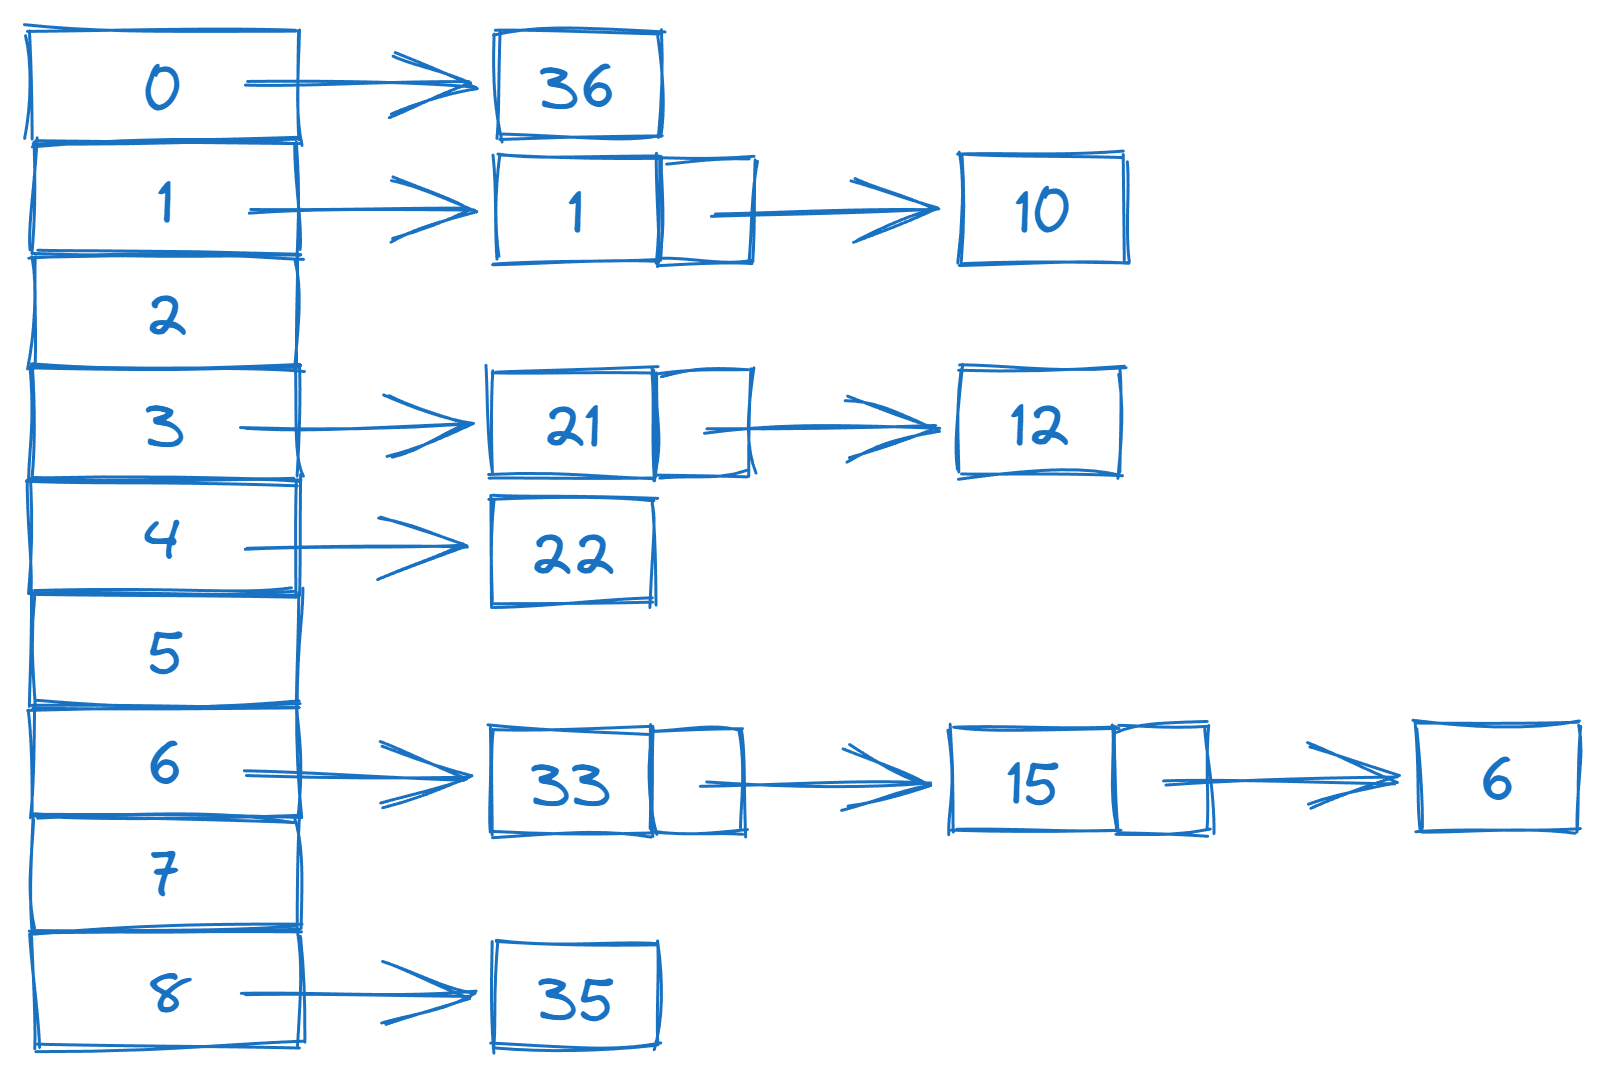
\includegraphics[width=0.5\linewidth]{HWs/HW6/figures/1.png}
    \label{fig:hash-table}
\end{figure}
